\documentclass[12pt,a4paper]{article}
\usepackage[UTF8]{ctex}
\usepackage{amsmath,amssymb}
\usepackage{booktabs}
\usepackage{float}
\usepackage{fancyhdr}   % 页眉页脚控制
\usepackage{geometry}
\usepackage{subfigure}  % 子图排版
\usepackage{subcaption}
\usepackage{graphicx}
\usepackage{listings} % 代码排版宏包
\usepackage{xcolor} % 代码高亮颜色
\usepackage{enumitem} % 列表格式控制宏包
\geometry{left=2.5cm,right=2.5cm,top=2.5cm,bottom=2.5cm}

\pagestyle{fancy}
\fancyhf{} % 清空默认页眉页脚
\fancyhead[L]{\small 分光仪的调节与使用}       % 左上角页眉
\fancyhead[R]{\small 2513318}          % 右上角章节名
\fancyfoot[C]{\thepage}                   % 居中页码（页脚）
\renewcommand{\headrulewidth}{0.4pt}      % 页眉线粗细
\renewcommand{\footrulewidth}{0.4pt}      % 页脚线粗细
%报告开始
\begin{document}
	%设置课程标题
	\begin{center}
		\heiti\LARGE{《大学基础物理实验》课程实验报告}
	\end{center}
	%设置实验人信息以及实验时间表格
	\begin{center}
		\begin{tabular}{lcr}
			{\songti 姓名及学号：陈秋实2513318}  \quad 专业：密码科学与技术 \quad 组别：L组1号 \\
			{\songti  学院：密码与网络空间安全学院 \quad 实验时间：2026年5月8日~星期五~下午}\\
		\end{tabular}
	\end{center}
	\vspace{-0.2cm}
	{\noindent}	 \rule[-10pt]{16cm}{0.05em}\\
	\vspace{-0.4cm}
	%实验题目
	\begin{center}
		\LARGE\textbf{分光仪的调节与使用}
	\end{center}

	
	
	\section{实验目的}
	\par 1.了解分光仪的结构和原理。
	\par 2.掌握分光仪的调节和使用方法。
	
	
    \section{实验原理}
    分光仪又称分光计，是用来测量光束偏转角的精密仪器，它可以精确地测量平行光的偏转角，是光学实验中一种常用的仪器。\textbf{其基本原理是}，让光线通过狭缝和聚焦透镜形成一束平行光线，经过反射或折射后进入望远镜物镜并成像在望远镜的焦平面上，通过目镜进行观察和测量各种光线的偏转角度，从而得到光学参量等。分光仪结构复杂、构件精密、调节要求高，调整操作技术较复杂，使用时必须按要求仔细调整，才能获得较高精度的实验结果。对初学者有一定难度，需要了解其结构和光路，严格按要求步骤耐心调节。
    
    由于分光仪对角度的测量精度较高，它有时也作为一种用光学方法测量角度的精密仪器。在光学实验中常用来测定光线的方向及各种角度。由于有些物理量如折射率、光栅常数、色散率等往往可以通过直接测量有关的角度（如最小偏向角、衍射角、布儒斯特角等）来确定，所以在光学技术中，分光仪的应用十分广泛。

	
	\section{实验仪器用具}
	如图1及图2所示
	\begin{figure}[!htbp]
		\centering
		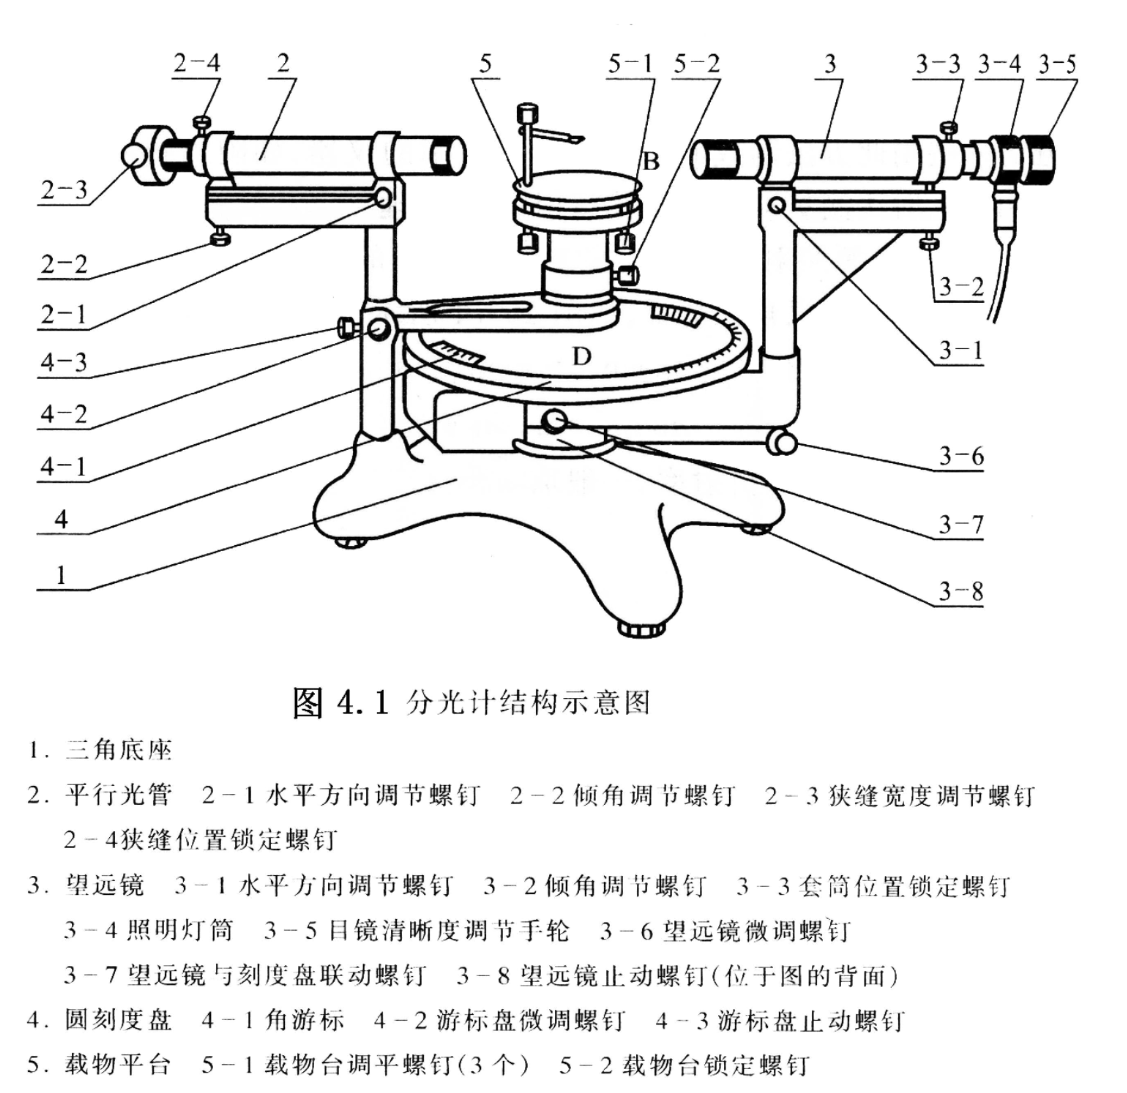
\includegraphics[width=0.9\textwidth]{分光仪.png}
		\caption{分光仪结构示意图}
	\end{figure}
	
	\begin{figure}[!htbp]
		\centering
		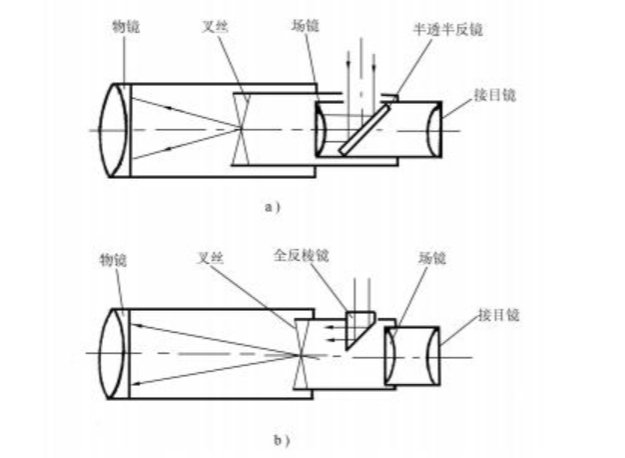
\includegraphics[width=0.7\textwidth]{望远镜.png}
		\caption{望远镜结构示意图}
	\end{figure}

	\section{实验步骤或内容}
	\par 打开所有的灯光，调节设备使得有成像。
	\subsubsection*{粗调}
	\par 从正面和上面观察装置，使得望远镜和平行光管刚好在同一条直线上。
	\subsubsection*{利用自准法将望远镜调焦于无穷远处}
	\par 载物台上放有一块半透半反镜，会将叉丝像反射。调节平面反射镜和望远镜的俯仰使得从望远镜中能看到反射回来的叉丝像，此时对望远镜进行调焦，使得返回的叉丝像变得清晰，并且与叉丝之间没有视差的时候，叉丝与叉丝像都位于望远镜物镜的焦平面上。
	\subsubsection*{用各半调节法使望远镜的光轴与仪器转轴垂直}
	\par 完成第二步调节后，进一步调节反射镜和望远镜的俯仰将叉丝像和叉丝重合。这时不能说明望远镜的光轴和仪器的中心转轴相互垂直。将平面镜旋转一百八十度，有可能出现在望远镜里看不到反射回来的叉丝像的现象，这时应当，这时应当调节俯仰，使得叉丝像在旋转前后都在望远镜内。再次将平面反射镜一面反射的叉丝像与叉丝调节重合，将平面镜翻转180度之后，发现叉丝像跟叉丝调节偏差了$d$的距离，调节望远镜的俯仰使得反射叉丝像向叉丝移动$\frac{d}{2}$的距离。在此之后，再调节反射镜的俯仰，使反射叉丝像和叉丝重合。事实上需要重复几次，因为目测很难确定$\frac{d}{2}$的位置。
	\subsubsection*{使得平行光管射出平行光，调节其光轴和仪器垂直}
	\par 调节狭缝与平行光管物镜之间的距离，直至能从望远镜中观察到边缘清晰，而且与叉丝之间无视差的狭缝像，再次调节平行光管的俯仰，使得狭缝上下对称与望远镜视场的中心的水平叉丝。
	
	
	\section{实验数据记录及处理}
	\begin{table}[htbp]
		\centering
		\caption{分光仪调节和使用实验数据记录表}
		\begin{tabular}{|c|c|c|c|c|}
			\hline
			游标号 & 望远镜筒位置 1 & 望远镜筒位置 2 & 望远镜筒转过的角度 & 消偏心差角度 \\
			\hline
			1 & $131^\circ 01'$ & $197^\circ 47'$ & $66^\circ 46'$ & $33^\circ 23'$ \\
			\hline
			2 & $311^\circ 01'$ & $17^\circ 49'$ & $66^\circ 48'$ & $33^\circ 24'$ \\
			\hline
		\end{tabular}
	\end{table}
	
	
	\section{实验结果及讨论}
	\textbf{测量方法评价：}使用分光仪测量角度精度较高，且采用对径双游标读数法有效消除了偏心差带来的系统误差。但该方法操作复杂，调节过程耗时较长，且对操作者的耐心和技术要求较高。\par
	\textbf{实验过程困难：}想要使绿叉的成像在正反两面都位于指定位置较为困难，需要反复进行细致的调整
\end{document}